\documentclass[handout]{beamer}
\mode<presentation> {%
	\usetheme[]{Boadilla}
	\usecolortheme{orchid}
	\setbeamercovered{transparent}
	\setbeamersize{text margin left=0.7cm}
  \setbeamersize{text margin right=0.7cm}
  \setbeamertemplate{enumerate item}[square]
  \setbeamertemplate{enumerate subitem}[circle]
  \setbeamertemplate{enumerate subsubitem}[>]
  \setbeamertemplate{itemize item}[square]
  \setbeamertemplate{itemize subitem}[circle]
  \setbeamertemplate{itemize subsubitem}[>]
}


\usepackage{bm}
\usepackage[utf8]{inputenc}
\usepackage[spanish]{babel}
\usepackage{times}
\usepackage[T1]{fontenc}
\usepackage{graphicx}
\usepackage{multirow}
\usepackage{pifont}
\usepackage{rotating}
\usepackage{colortbl}
\usepackage[framed]{mcode}
\usepackage{verbatim}
\usepackage{mathtools}
% \usepackage{tikz}
% \usetikzlibrary{positioning}
% \usetikzlibrary{shapes.multipart,decorations.pathreplacing}
% \tikzstyle{bloque}=[rectangle,rounded corners=2pt,draw=black!60,fill=black!5,very thick,minimum size=5mm,align=center]%
% \tikzstyle{arrow}=[very thick,color=black!60]%


\definecolor{olivegreen}{rgb}{0.0,0.5,0.0}
% \definecolor{general}{rgb}{0.9 0.9 1}%
% \newrgbcolor{colorsistema}{0 1 1}
% \newrgbcolor{colorviolet}{0.9 0.8 1}

\author[J. Chacón]{%[Author, Another] % (optional, use only with lots of authors)
\textit{Ingeniería Electrónica de Comunicaciones }\\
\vspace{0.6cm}
\small Jesús Chacón Sombría}%\inst{1} \and S.~Another\inst{2}}


\institute[DACYA. UCM] % (optional, but mostly needed)
{
  %\inst{1}%

\footnotesize  Departamento de Arquitectura de Computadores y Automática.\\
  Universidad Complutense de Madrid
  }

\date[Diseño de filtros] % (optional)
{\footnotesize Curso 2025-2026}%{\today / Master}
\subject{Talks}

\pgfdeclareimage[height=0.75cm]{logo}{ucm}

\usepackage[absolute,overlay]{textpos}
\setlength{\TPHorizModule}{1mm}
\setlength{\TPVertModule}{1mm}
\newcommand{\MyLogo}{%
\begin{textblock}{14}(116.0,0.6)
  \pgfuseimage{logo}
\end{textblock}
}

\makeatletter
\numberwithin{section}{part}
\AtBeginPart{
\beamer@tocsectionumber=0\relax
\frame{\partpage}
}
\makeatother

\begin{document}

\begin{frame}
  \titlepage
\end{frame}

\newcommand*\oldmacro{}%
\let\oldmacro\insertshorttitle%
\renewcommand*\insertshorttitle{%
 \MyLogo
  \oldmacro\hfill%
}

\AtBeginSection[]{}
\AtBeginSubsection[]{}

\subsection{Filtros FIR}

\begin{frame}
  \frametitle{Filtros FIR de fase lineal}
  \[
  H(\mathrm{e}^{j\omega})=\substack{N-1\\\sum\\n=0}h[n]\mathrm{e}^{-j\omega n}
  \]
  \vspace{0.1cm}

  \alert{¿Podemos garantizar por diseño un filtro FIR de fase lineal?}
  
  \begin{itemize}
    \footnotesize
    \item Consideramos FIR con $h[n]$ real: $\color{blue}h[n] = h^*[n]\Leftrightarrow H(e^{j\omega})=H^*(e^{-j\omega})$.
    \item Un FIR con fase lineal tiene simetría par o impar $\color{blue}h[n]=\pm h[N-1-n]$.
    \hspace*{-1.25cm}\begin{minipage}{0.8\textwidth}
      \scriptsize
      \[\begin{aligned}
      \substack{N-1\\\sum\\n=0}h[n]\mathrm{e}^{-j\omega n}&=
      \substack{N-1\\\sum\\n=0}h[N-1-n]\mathrm{e}^{j\omega n}
      =h[0] + h[1]\mathrm{e}^{-j\omega} + ... + h[N-1] \mathrm{e}^{-j\omega (N-1)}\\
      &=\mathrm{e}^{-j\omega\frac{N-1}{2}}(h[0]\mathrm{e}^{j\omega\frac{N-1}{2}} + h[1]\mathrm{e}^{j\omega(\frac{N-1}{2} - 1)} + ... + h[N-1] \mathrm{e}^{-j\omega\frac{N-1}{2}})\\
      &=\left\{\begin{matrix*}[l]
        \mathrm{e}^{-j\omega\frac{N-1}{2}}\left(\substack{N/2-1\\\sum\\n=0}h[n](\mathrm{e}^{j\omega (\frac{N-1}{2} - n)}\pm\mathrm{e}^{-j \omega (\frac{N-1}{2} - n)})\right) & \mathrm{si}~N~\mathrm{es~par}\\[2ex]
        \mathrm{e}^{-j\omega\frac{N-1}{2}}\left(h[\frac{N-1}{2}] + \substack{(N-3)/2\\\sum\\n=0}h[n](\mathrm{e}^{j\omega (\frac{N-1}{2} - n)}\pm\mathrm{e}^{-j \omega (\frac{N-1}{2} - n)})\right) & \mathrm{si}~N~\mathrm{es~impar}
      \end{matrix*}\right.
      \end{aligned}
      \]
    \end{minipage}
    \item $\color{blue}H(\mathrm{e}^{j\omega})=\mathrm{e}^{j\beta}\mathrm{e}^{-j\omega\frac{N-1}{2}}\hat H(\mathrm{e}^{j\omega})$, con $\hat H(\mathrm{e}^{\omega})$ una función real (\alert{la respuesta deseada}).
  \end{itemize}
\end{frame}

\begin{frame}
  \frametitle{Filtros FIR de fase lineal}
  \[
  H(\mathrm{e}^{j\omega})=\substack{N-1\\\sum\\n=0}h[n]\mathrm{e}^{-j\omega n}
  \]
  \vspace{0.1cm}

  \alert{¿Podemos garantizar por diseño un filtro FIR de fase lineal?}
  
  \begin{itemize}
    \footnotesize
    \item Un FIR con fase lineal tiene simetría par o impar $\color{blue}h[n]=\pm h[N-1-n]$.
    \hspace*{-1.25cm}\begin{minipage}{0.8\textwidth}
      \scriptsize
      \[
        H(\mathrm{e}^{j\omega})=\left\{\begin{matrix*}[l]
        \mathrm{e}^{-j\omega\frac{N-1}{2}}\left[h[L] + \substack{(N-3)/2\\\sum\\n=0}2\cdot h[n]\cdot\mathrm{cos}(\omega(L-n))\right] & h[n]=+h[N-1-n],N~\mathrm{impar} \\[2ex]
        \mathrm{e}^{-j\omega\frac{N-1}{2}}\left[\substack{N/2-1\\\sum\\n=0}2\cdot h[n]\cdot\mathrm{cos}(\omega(L-n))\right] & h[n]=+h[N-1-n],N~\mathrm{par} \\[2ex]
        j\mathrm{e}^{-j\omega\frac{N-1}{2}}\left[\substack{(N-3)/2\\\sum\\n=0}2\cdot h[n]\cdot\mathrm{sin}(\omega(L-n))\right] & h[n]=-h[N-1-n],N~\mathrm{impar} \\[2ex]
        j\mathrm{e}^{-j\omega\frac{N-1}{2}}\left[\substack{N/2-1\\\sum\\n=0}2\cdot h[n]\cdot\mathrm{sin}(\omega(L-n))\right] & h[n]=-h[N-1-n],N~\mathrm{par}
      \end{matrix*}\right.
      \]
    \end{minipage}
    \item $\color{blue}H(\mathrm{e}^{j\omega})=\mathrm{e}^{j\beta}\mathrm{e}^{-j\omega\frac{N-1}{2}}\hat H(\mathrm{e}^{j\omega})$, con $\hat H(\mathrm{e}^{\omega})$ una función real (\alert{la respuesta deseada}).
  \end{itemize}
\end{frame}


\begin{frame}
  \frametitle{Filtros FIR de fase lineal}
 
  \alert{¿Podemos garantizar por diseño un filtro FIR de fase lineal?}
  
  \begin{itemize}
    \footnotesize %\mathrm{e}^{-j\frac{\omega N}{2}}
    \item \alert{Tipo 1}: simetría par $h[n]=h[N-1-n]$, $N$ impar:\\
    \[
    \hat H(\mathrm{e}^{j\omega})=h[\frac{N-1}{2}] + \sum_{n=0}^{\frac{N-3}{2}}2\cdot h[n]\cdot\mathrm{cos}\left[\omega\left(\frac{N-1}{2}-n\right)\right]
    \]
    \item \alert{Tipo 2}: simetría par $h[n]=h[N-1-n]$, $N$ par:
    \[
    \hat H(\mathrm{e}^{j\omega})=\sum_{n=0}^{\frac{N}{2}-1}2\cdot h[n]\cdot\mathrm{cos}\left[\omega\left(\frac{N-1}{2} - n\right)\right]
    \]
    \item \alert{Tipo 3}: simetría impar $h[n]=-h[N-1-n]$, $N$ impar:
    \[
    \hat H(\mathrm{e}^{j\omega})=\sum_{n=0}^{\frac{N-3}{2}}2\cdot h[n]\cdot\mathrm{sin}\left[\omega\left(\frac{N-1}{2} - n\right)\right],~h[L]=0
    \]
    \item \alert{Tipo 4}: simetría impar $h[n]=-h[N-1-n]$, $N$ par:
    \[
    \hat H(\mathrm{e}^{j\omega})=\sum_{n=0}^{\frac{N}{2}-1}2\cdot h[n]\cdot\mathrm{sin}\left[\omega\left(\frac{N-1}{2} - n\right)\right]
    \]
  \end{itemize}
\end{frame}


\begin{frame}
  \frametitle{Filtros FIR de fase lineal}

  \alert{Diseño por muestreo en frecuencia}
  \begin{itemize}
    \item Podemos especificar $\hat H(\mathrm{e}^{j\omega})$ en un conjunto de frecuencias.
    \begin{itemize}
      \item Tipos 1 y 2, en $\hat H(\omega_n)$ para $\omega_n=\frac{2\pi n}{N}$.
      \item Tipos 3 y 4, en $\hat H(\omega_n)$ para $\omega_n=\frac{2\pi (n+1/2)}{N}$.
    \end{itemize}

    \item P.ej. para tipo 1 se obtiene $\hat H(\frac{2\pi n}{N})$ para $n=0,1,...,L$:
    \[
      \left[\begin{matrix}
        H(\omega_0)\\
        ...\\
        H(\omega_{L})
      \end{matrix}\right]=
      \left[\begin{matrix}
        \mathrm{cos}(\omega_0 L) & ... & \mathrm{cos}(\omega_0 (L-n)) \\
        ... & ... & ... \\
        \mathrm{cos}(\omega_1 L) & ... & \mathrm{cos}(\omega_L (L-n))
      \end{matrix}\right]
      \left[\begin{matrix}
       h[0]\\
       ...\\
       h[L]
      \end{matrix}\right]
    \]
    \item Y resolviendo se obtienen los coeficientes del filtro, $h[n]$.
  \end{itemize}
\end{frame}


\begin{frame}
  \frametitle{Filtros FIR de fase lineal}
  \footnotesize
  \begin{itemize}
    \item Localización de los ceros:
    \begin{itemize}
    \footnotesize
    \item $h[n]$ es real, tiene las raíces (ceros) reales o complejas conjugadas.
    \vspace{0.1cm}  
    \item \color{blue}$h[n]=+h[N-n] \rightarrow H(z)=+z^{-N}H(z^{-1})$\color{black}\\
    \vspace{0.1cm}
    {\scriptsize\color{teal} $H(z)=\sum_{n=0}^N h[n]z^{-n}=\sum_{n=0}^N h[N-n]z^{-n}=\sum_{m=0}^N h[m]z^{-N+m}$}\\
    \vspace{0.1cm}
    \item \color{blue}$h[n]=-h[N-n] \rightarrow H(z)=-z^{-N}H(z^{-1})$\color{black}\\
    \vspace{0.1cm}    
    {\scriptsize\color{teal} $H(z)=\sum_{n=0}^N h[n]z^{-n}=-\sum_{n=0}^N h[N-n]z^{-n}=-\sum_{m=0}^N h[m]z^{-N+m}$}

    \vspace{0.2cm}
    \item Como $z=re^{j\theta}$ y $z^{-1}=\frac{1}{r}e^{-j\theta}$, los ceros de los FIR de fase lineal representan una simetría especular respecto al círculo unidad.
    
    \end{itemize}
    \item Los cuatro tipos de filtros se diferencian en los ceros que hay en +1 y -1.
    \begin{itemize}
      \scriptsize
      \item \alert{Tipo 1 (N par): Un número par o ningún cero en +1 y -1.}
      \item \alert{Tipo 2 (N impar): Un número par o ningún cero en +1 y un número impar en -1.}
      \item \alert{Tipo 3 (N par): Un número impar en +1 y -1.}
      \item \alert{Tipo 4 (N impar): Un número impar +1 y un número par o ninguno en -1.}
    \end{itemize}
  \end{itemize}
\end{frame}
  
\begin{frame}
  \frametitle{Filtros FIR de fase lineal}
  \footnotesize

  \begin{tabular}{c>{\columncolor{yellow}}c>{\columncolor{lime}}c}
    \rowcolor{white} 
    & \color{black}\tiny \color{blue}Simetría par $h[n]=h[N-1-n]$\color{black} & \color{black}\tiny \color{blue}{Simetría impar $h[n]=-h[N-1-n]$}\\
    \rotatebox{90}{\color{blue}\small $N$ par\color{black} $\quad$}    & \parbox{5cm}{\centering Tipo 1\\{\tiny \alert{Nº par de ceros en +1 y Nº par de ceros en -1}}\\[1ex]\tiny$\hat H(\mathrm{e}^{j\omega})=h[L] + \sum_{n=0}^{L-1}2\cdot h[n]\cdot\mathrm{cos}(\omega (L-n))$\\[2ex]} & \parbox{5cm}{\centering Tipo 3\\\alert{\tiny Nº impar de ceros en +1 y Nº impar de ceros en -1}\\[1ex]\tiny$\hat H(\mathrm{e}^{j\omega})=\sum_{n=0}^{L-1}2\cdot h[n]\cdot\mathrm{sin}(\omega (L - n)),~h[L]=0$\\[2ex]} \\
    \rotatebox{90}{\centering\color{blue}\small $N$ impar\color{black} $\quad$}  & \parbox{5cm}{\centering Tipo 2\\\alert{\tiny Nº par de ceros en +1 y Nº impar de ceros en -1}\\[1ex]\tiny$\hat H(\mathrm{e}^{j\omega})=\sum_{n=0}^{L-1}2\cdot h[n]\cdot\mathrm{cos}(\omega (L - n))$\\[2ex]} & \parbox{5cm}{\centering Tipo 4\\\alert{\tiny Nº impar de ceros en +1 y Nº par de ceros en -1}\\[1ex]\tiny$\hat H(\mathrm{e}^{j\omega})=\sum_{n=0}^{L-1}2\cdot h[n]\cdot\mathrm{sin}(\omega (L - n))$\\[2ex]} \\
  \end{tabular}  
\end{frame}



\begin{frame}
  \frametitle{Filtros de fase 0} 
  \vspace{-0.2cm}
  \begin{itemize}
  \footnotesize
    \item Un filtro de de fase 0 es aquel que tiene una $H(e^{j\omega})$ real y no negativa.    % \item Se puede implementar como  $H(z)=F(z)F(z^{-1})$, donde  F(z) es un sistema que no tiene polos sobre el círculo unidad. 
    \item Por construcción, $H(z)=F(z)F(z^{-1})$, es un filtro de fase 0:
  $H(e^{j\omega})=H(z=e^{j\omega})=F(e^{j\omega})F(e^{-j\omega})=|F(e^{j\omega})|^2$, es real positivo.
    \item Los polos y ceros tienen simetría especular respecto al circulo unidad.  
    \item Es inestable, pero se puede aplicar a una señal de longitud finita:

    \begin{columns}[T]
      \begin{column}{4cm}  
        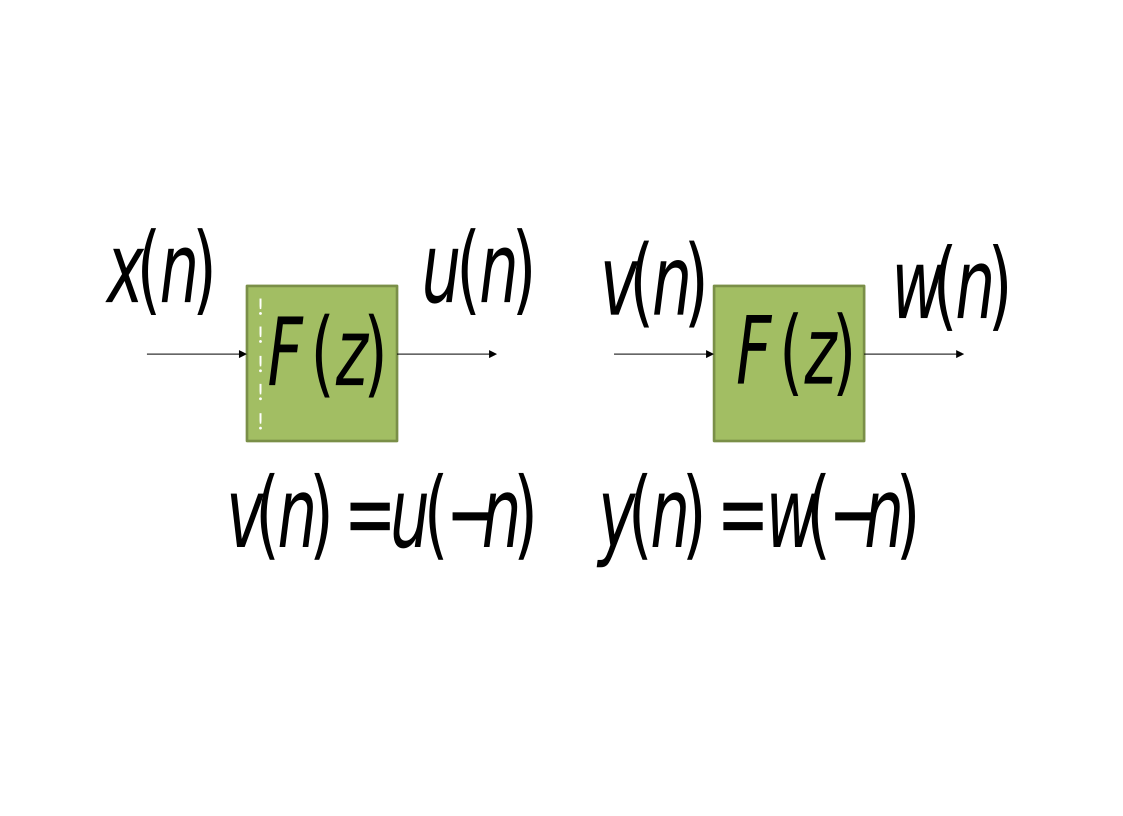
\includegraphics[trim=4cm 1cm 4cm 1cm,width=4cm, height=2.5cm]{Figures/FiltroFase0}
      \end{column}
      \begin{column}{4cm}
      
      $Y(e^{jw})=W^*(e^{jw})=F^*(e^{jw})V^*(e^{jw})=F^*(e^{jw})U(e^{jw})=F^*(e^{jw})F(e^{jw})X(e^{jw})=|F(e^{jw})|^2X(e^{jw})$
      \end{column}
    \end{columns}
  
  \item En Matlab \color{blue}\texttt{y=filtfilt(Fnumz,Fdenz,x)}\color{black} hace un filtrado de fase 0.
  \end{itemize}
\end{frame}
  


\begin{frame}
  \frametitle{Filtros de fase mínima/máxima}
  \vspace{-0.2cm}
  \begin{itemize}
    \footnotesize
    \item Esta clasificación se basa en la posición de los ceros de un sistema.
    \item \color{olivegreen}Ejemplo: dos sistemas con el mismo polo y ceros invertidos
    \begin{itemize}
      \color{gray}
      \footnotesize
      \item $H_1(z)=\frac{z+b}{z+a}$   con $|a|<1$ y $|b|<1$  $\rightarrow Z_{POLO}=-a$ y  $Z_{CERO}=-b$
      \item $H_2(z)=\frac{bz+1}{z+a}$   con $|a|<1$ y $|b|<1$ $\rightarrow Z_{POLO}=-a$ y  $Z_{CERO}=-1/b$
      \vspace{0.1cm}
      $H_2(z)=\frac{bz+1}{z+a}\frac{z+b}{z+b}=\frac{z+b}{z+a}\frac{bz+1}{z+b}=H_1(z)H_{PasoTodas}(z)$
      \vspace{0.1cm}
      $H_2(e^{j\omega})=H_1(e^{j\omega})H_{PT}(e^{j\omega})$ 
      \vspace{0.1cm}
      \scriptsize
      \hspace{1cm}$\rightarrow |H_2(e^{j\omega})|=|H_1(e^{j\omega})||H_{PT}(e^{jw})|=|H_1(e^{j\omega})|$
      \vspace{0.1cm}
      \hspace{1cm}$\rightarrow arg(H_2(e^{j\omega}))=arg(H_1(e^{j\omega}))+arg(H_{PT}(e^{j\omega}))=$
      \vspace{0.1cm}
      \hspace{3.1cm}$=arg(H_1(e^{j\omega}))-\alpha(\omega)$ con $0<\alpha(\omega)<\pi$
      \color{black}
    \end{itemize}  
    \vspace{-0.3cm}  
    \color{black}
    \item Generalización:
    \begin{itemize}
      \scriptsize
      \item $H_{MIN}(z)$: FT causal estable con todos sus ceros dentro del círculo unidad
      \item $H_{MAX}(z)$: FT causal estable con todos sus ceros simétricos respecto al círculo unidad y el caso anterior
      \item $H_{MAX}(z)=H_{MIN}(z)H_{PasoTodas}(z)$ con $H_{PT}(z)$ filtro paso todo estable en base a los ceros de $H_{MIN}(z)$
      \item $|H_{MAX}(e^{j\omega})|=|H_{MIN}(e^{j\omega})|$
      \item $arg(H_{MAX}(e^{j\omega}))=arg(H_{MIN}(e^{j\omega}))-\alpha(w)$ con $0<\alpha(\omega)<N\pi$ y N el número de ceros del filtro.
    \end{itemize}
  \end{itemize}
\end{frame}
  
  
\begin{frame}
  \frametitle{Filtros Paso Todas}    
    \vspace{-0.2cm}    
    \begin{itemize}
      \footnotesize
      \item Un filtro paso todas cumple que : $|H(e^{jw})|=1 \:\: \forall w$    
      \item Un filtro IIR con coeficientes reales y causal de la forma
      
      $H(z)=\pm \frac{d_M + d_{M-1}z^{-1}+\dots+ z^{-M}}{1+d_1z^{-1}+\dots+ d_M z^{-M}}=\pm \frac{z^{-M}D_M(z^{-1})}{D_M(z)}$
      
      \hspace{4cm}$D_M(z)=1+d_1 z^{-1}+\dots + d_M z^{-M}$    
      \item Es por construcción un filtro paso todas:
      
      $|H(e^{jw})|^2\!=\!H(e^{jw})H(e^{-jw})\!=\!H(z)H(z^{-1})|_{z=e^{jw}}\!=\!(\pm)^2 \frac{z^{-M}D_M(z^{-1})}{D_M(z)} \frac{z^{M}D_M(z)}{D_M(z^{-1})}=1$    
      \item $z_{POLO}=re^{j\theta}  \leftrightarrow z_{CERO}=\frac{1}{r}e^{j\theta}$
      
      \item Si el filtro es estable $\rightarrow$ tiene sus polos (raíces de $D_M(z)$) dentro del círculo unidad y sus ceros (raíces de $D_M(z^{-1})$) fuera del círculo unidad. Los polos y los ceros se encuentran enfrentados con una simetría especular respecto al círculo.
      
      \item Como no atenúan ninguna frecuencia, son útiles para modificar el desfase introducido por otros filtros. 
      
      \item El desfase total introducido por el filtro paso todas H(z) entre las frecuencias $w\in[0 ,\pi]$ es de $M\pi$. 
    \end{itemize}
\end{frame}
  
\begin{frame}
  \frametitle{Filtros Combados}
  \begin{itemize}
    \footnotesize
    \item Partimos de un filtro de referencia: $\hat H(z)=\sum_{n=-\infty}^\infty \hat h[n]z^{-n}$.
    \item Hacemos una transformación espectral $\color{blue} z=z^L$:
    \vspace{-0.2cm}
    \[\color{blue}
    H(z)=\hat H(z^L)=\sum_{n=-\infty}^\infty \hat h[n]z^{-Ln}
    \]
    \vspace{-0.4cm}
    \item La respuesta en frecuencia periódica en $\omega$ con periodo $\frac{2\pi}{L}$.
    \vspace{-0.2cm}
    \[
    H(e^{j\omega})=\sum_{n=-\infty}^\infty\hat h[n]e^{-jLn\omega}=\hat H(e^{j\omega L})
    \]
    \vspace{-0.4cm}
    \item Diseño con Matlab de IIR combados:    
    \begin{itemize}\scriptsize
      \item \color{blue}\texttt{[num,den]=iircomb(L,Bw,tipo);}\color{black}
      \item $B_\omega$: ancho de banda de paso (normalizado)
      \item Tipo: 'peak', 'notch'
    \end{itemize}
  \end{itemize}
\end{frame}

\begin{frame}
  \frametitle{Ejemplos de FIR Combados}
  \footnotesize
  \color{olivegreen} Estudiar la respuesta en frecuencia que se obtiene al combar los siguientes filtros FIR:
  \begin{columns}[c]
    \begin{column}{4.5cm}
      \vspace{0.5cm}
      $G_1(z)=\frac{1}{2}(1+z^{-1})$
      \vspace{0.2cm}
      $G_2(z)=\frac{1}{3}(1+z^{-1}+z^{-2})$
      \vspace{1.3cm}
      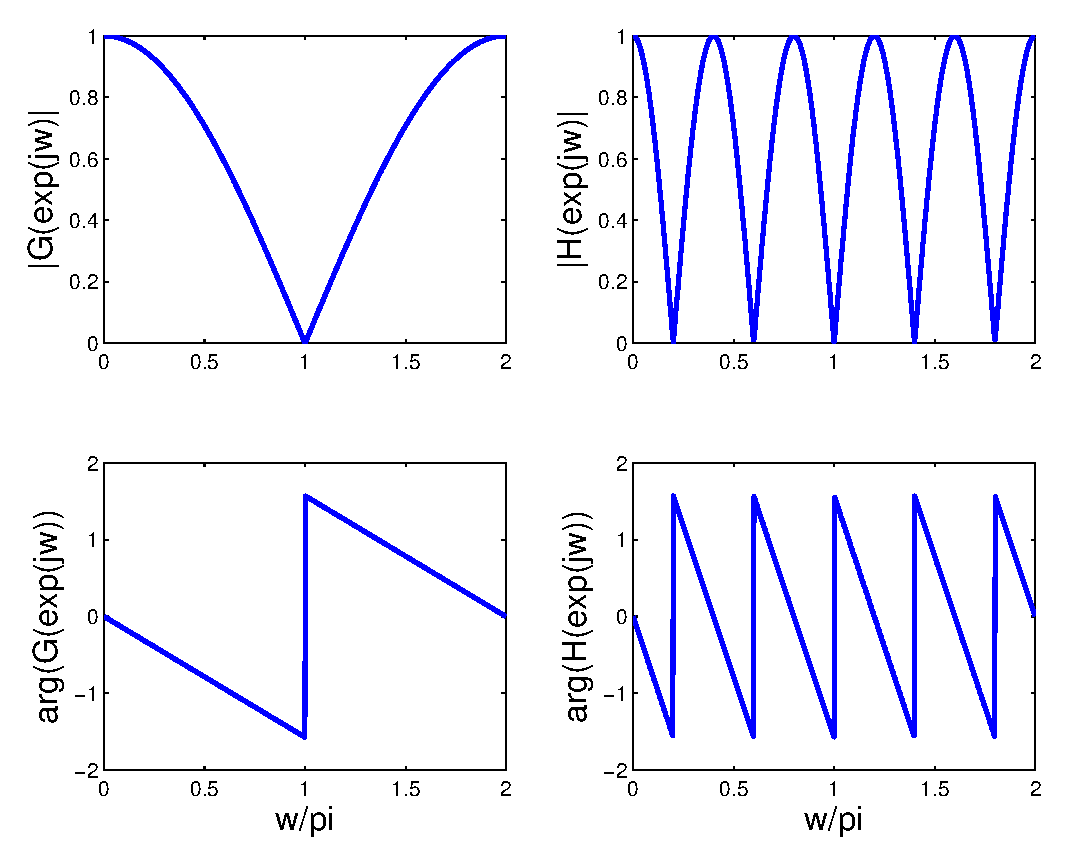
\includegraphics[width=4cm]{./Figures/EjCombFir2.eps}
      \color{gray}
      \hspace{1.5cm}$G_1(z)$
    \end{column}
    \begin{column}{5cm}
      \color{gray}
      \lstinputlisting{./Matlab/EjCombFIR.m}
      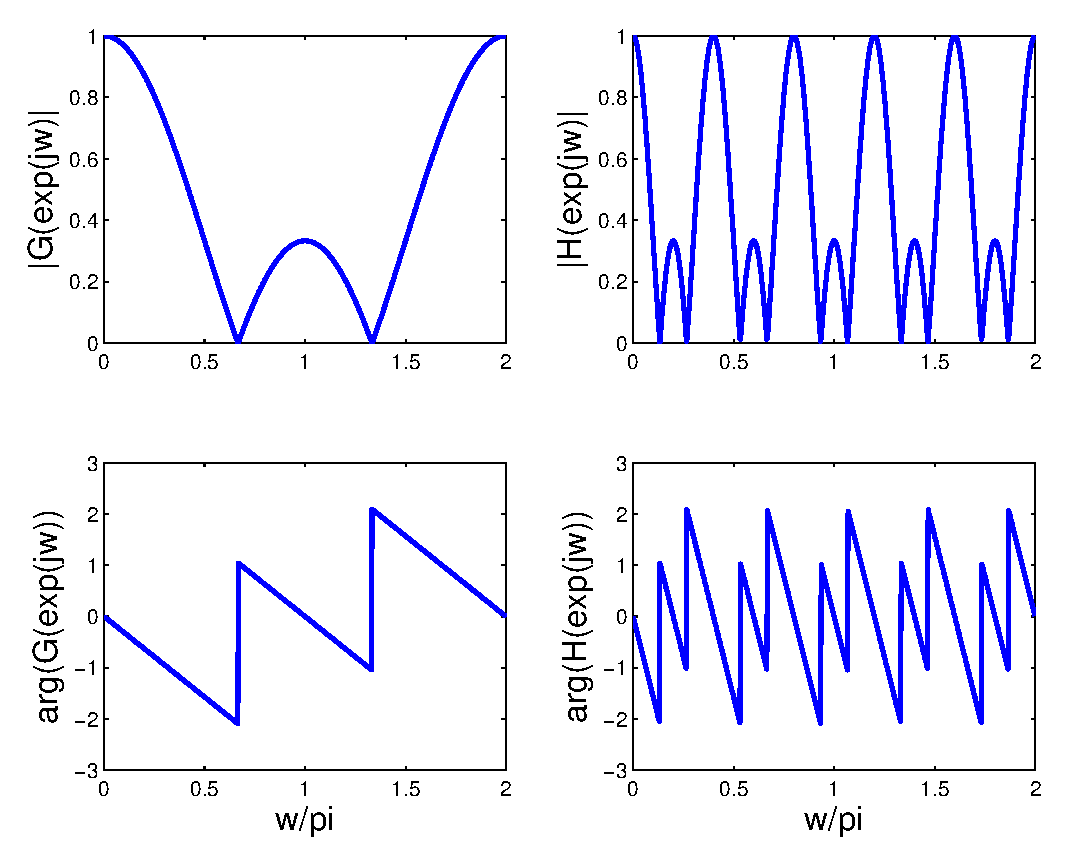
\includegraphics[width=4cm]{./Figures/EjCombFir3.eps}
      \hspace{1.5cm}$G_2(z)$
    \end{column}
  \end{columns}
\end{frame}

\begin{frame}
  \frametitle{Ejemplos de IIR Combados con Matlab}
  \footnotesize 
  \color{olivegreen} Deseamos diseñar un filtro combado para eliminar un ruido 
  eléctrico generado por la red de suministro a $f_0=50Hz$ y sus armónicos.
  para un sistema muestreo a $f=5kHz$.

  \vspace{0.5cm}
  \begin{columns}[c]
    \begin{column}{0.5\textwidth}
      \color{black}
      $\omega_d=\omega_cT_s=2\pi \frac{f_0}{f_s}=\frac{2\pi}{L}$\\
      $\rightarrow L=\frac{f_s}{f_{0}}=50,~B_{\omega, max}=\frac{2\pi}{L}=0.314$
      \lstinputlisting{./Matlab/EjCombIIRMatlab.m}
    \end{column}
    \begin{column}{0.5\textwidth}
      \color{gray}
      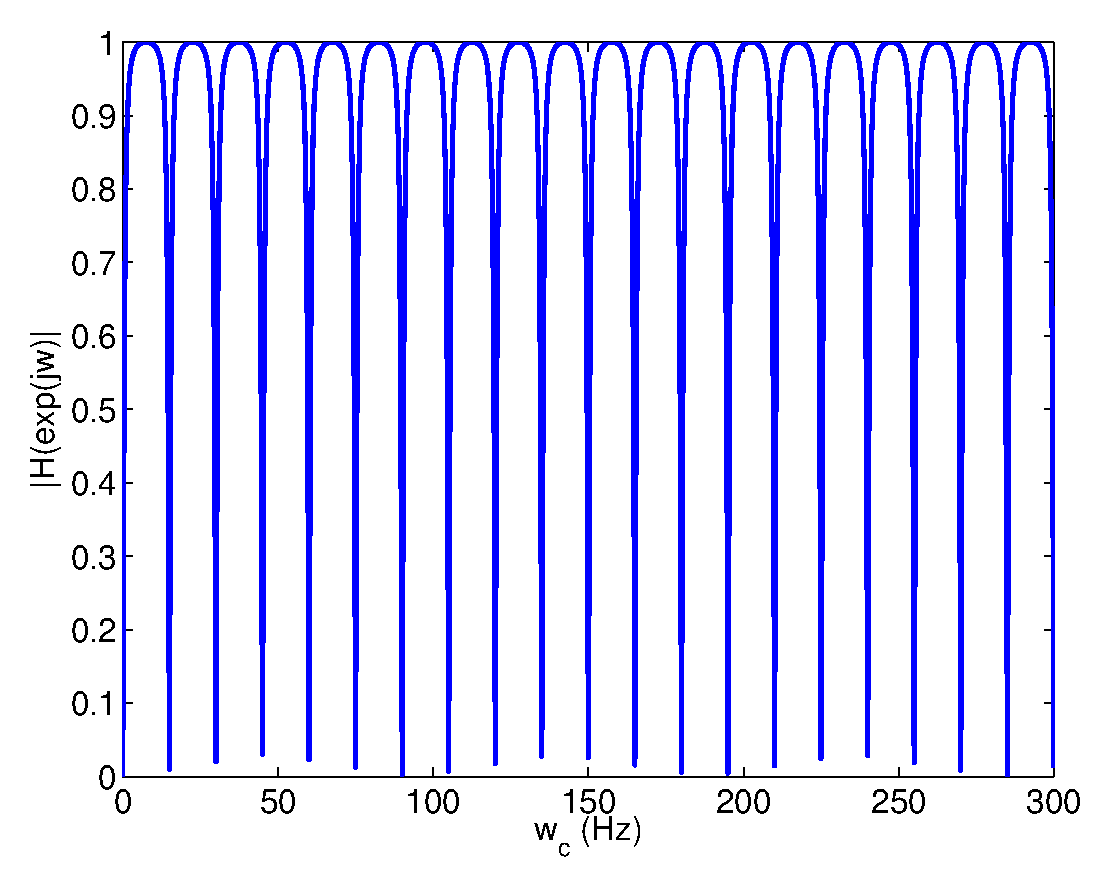
\includegraphics[width=5.5cm]{./Figures/EjCombIIRMatlab.eps}
    \end{column}
  \end{columns}
\end{frame}
  
\end{document}
